% Short overview rebuilt from complementary/other-slides/a.11.a-misp-data-model-overview.pdf.
\documentclass[aspectratio=169]{beamer}
\usetheme[numbering=progressbar]{misp}
\usepackage[utf8]{inputenc}
\usepackage[T1]{fontenc}
\usepackage{booktabs}
\usepackage{array}
\usepackage{tikz}
% Shared MISP identity palette; usable in Beamer and standalone diagrams.
\usetikzlibrary{arrows.meta,positioning,fit,backgrounds,calc}
\definecolor{dmNavy}{HTML}{02394A}
\definecolor{dmTeal}{HTML}{00708D}
\definecolor{dmBlue}{HTML}{0091B0}
\tikzset{
  dm box/.style={draw=dmTeal,fill=dmBlue!6,rounded corners=3pt,
    text=dmNavy,font=\sffamily\small,align=center,inner sep=7pt,
    text width=3.35cm,minimum height=1cm,
    execute at begin node={\hyphenpenalty=10000\relax}},
  dm title/.style={dm box,fill=dmNavy,text=white,font=\sffamily\small\bfseries},
  dm label/.style={font=\sffamily\scriptsize,text=dmNavy,align=center,
    fill=white,inner sep=3pt},
  dm arrow/.style={-{Stealth[length=2.2mm]},thick,draw=dmTeal},
  dm match/.style={{Stealth[length=2mm]}-{Stealth[length=2mm]},
    thick,dashed,draw=dmTeal},
  dm group/.style={draw=dmTeal,rounded corners=5pt,fill=dmBlue!3,inner sep=12pt}
}

\newcolumntype{L}[1]{>{\raggedright\arraybackslash}p{#1}}
\renewcommand{\arraystretch}{1.15}

\title{MISP data model overview}
\subtitle{Structure, context, relationships and feedback}
\author{\texorpdfstring{Team CIRCL \\ \emph{TLP:CLEAR}}{Team CIRCL (TLP:CLEAR)}}
\institute{MISP Project \\ \url{https://www.misp-project.org/}}
\date{Reference: 7 November 2026 --- MISP 2.5}

\begin{document}
\begin{frame}[t,plain]
  \titlepage
  \note{A short conceptual overview for analysts and integrators. Allow 25--35 minutes,
  including the exercise. Adapted from the 19-page complementary overview, reviewed
  against MISP 2.5.51 source on 7 November 2026. All diagrams are editable TikZ.
  The examples use reserved domains and documentation IP addresses.}
\end{frame}

\begin{frame}{Read the model in four parts}
  \begingroup\centering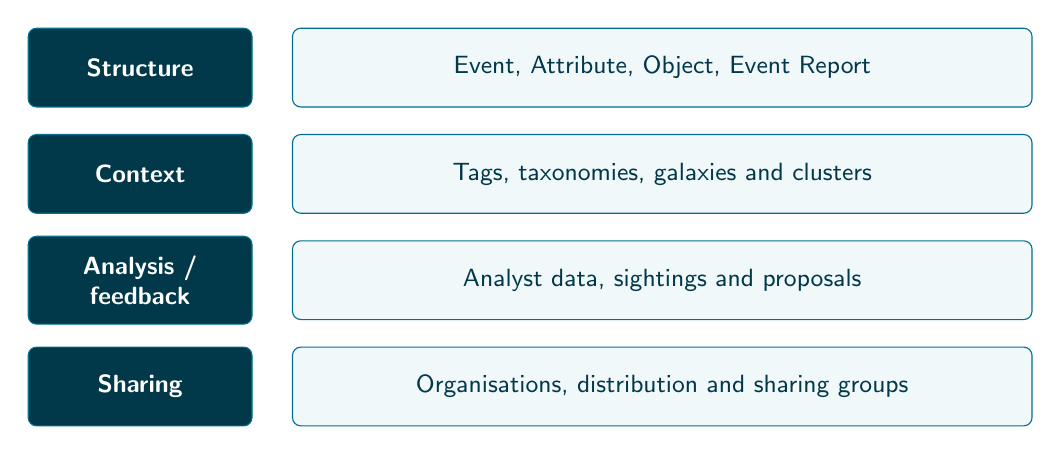
\begin{tikzpicture}
  \node[dm title,text width=2.35cm] (data) at (0,0) {Structure};
  \node[dm box,text width=8.9cm,right=5mm of data] {Event, Attribute, Object, Event Report};
  \node[dm title,text width=2.35cm] (context) at (0,-1.35) {Context};
  \node[dm box,text width=8.9cm,right=5mm of context] {Tags, taxonomies, galaxies and clusters};
  \node[dm title,text width=2.35cm] (feedback) at (0,-2.7) {Analysis / feedback};
  \node[dm box,text width=8.9cm,right=5mm of feedback] {Analyst data, sightings and proposals};
  \node[dm title,text width=2.35cm] (sharing) at (0,-4.05) {Sharing};
  \node[dm box,text width=8.9cm,right=5mm of sharing] {Organisations, distribution and sharing groups};
\end{tikzpicture}
\par\endgroup
  \note{These are teaching groups, not separate databases or an exhaustive schema.
  Structure holds observations and narrative; context classifies and identifies
  concepts; feedback adds analysis; sharing determines availability. References and
  correlations connect data across these views. Proposals are change suggestions
  (ShadowAttribute), distinct from analyst data.}
\end{frame}

\begin{frame}{An event is a contextual envelope}
  \begingroup\centering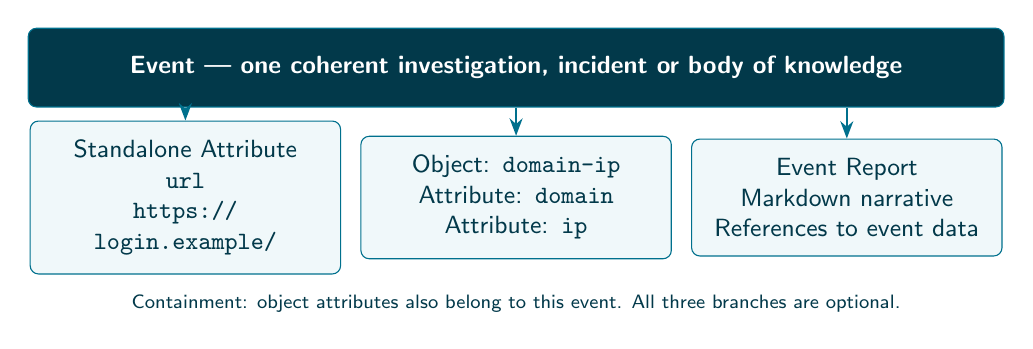
\begin{tikzpicture}
  \node[dm title,text width=11.9cm] (event) at (0,0)
    {Event --- one coherent investigation, incident or body of knowledge};
  \node[dm box,text width=3.45cm] (attr) at (-4.2,-1.65)
    {Standalone Attribute\\\texttt{url}\\\texttt{https://}\\\texttt{login.example/}};
  \node[dm box,text width=3.45cm] (object) at (0,-1.65)
    {Object: \texttt{domain-ip}\\Attribute: \texttt{domain}\\Attribute: \texttt{ip}};
  \node[dm box,text width=3.45cm] (report) at (4.2,-1.65)
    {Event Report\\Markdown narrative\\References to event data};
  \draw[dm arrow] (event.south -| attr.north) -- (attr.north);
  \draw[dm arrow] (event.south) -- (object.north);
  \draw[dm arrow] (event.south -| report.north) -- (report.north);
  \node[dm label] at (0,-3.0) {Containment: object attributes also belong to this event. All three branches are optional.};
\end{tikzpicture}
\par\endgroup
  \begin{itemize}
    \item Event metadata records identity, creator, date and analysis state.
    \item Distribution and sharing groups help define the audience.
  \end{itemize}
  \note{Containment arrows do not mean automatic copying of tags to every child.
  Org is the local owner and Orgc the creating organisation; these can differ after
  synchronisation. An event may describe an incident, campaign, report or another
  coherent topic. It need not contain every kind of element. An unpublished event
  can still be visible to authorised readers: publication is not confidentiality.}
\end{frame}

\begin{frame}{Attributes are typed data points}
  \begin{columns}[T,onlytextwidth]
    \column{.48\textwidth}
    \begin{block}{A standalone attribute}
      \texttt{type: domain}\\
      \texttt{value: login.example}\\
      \texttt{category: Network activity}\\
      \texttt{to\_ids: false}
    \end{block}
    \column{.48\textwidth}
    \begin{itemize}
      \item Type gives the value its meaning.
      \item UUID identifies this attribute.
      \item Comments and observation times add detail.
      \item Tags and distribution add context and sharing controls.
    \end{itemize}
  \end{columns}
  \medskip
  \texttt{to\_ids} signals intended detection use; assess confidence and freshness separately.
  \note{An attribute can represent an indicator or supporting information. Types include
  domain, ip-dst, sha256, attachment and many others. first\_seen and last\_seen describe
  observation time; timestamp records modification. to\_ids does not define access,
  truth or correlation eligibility. Do not repeat the old blanket rule that attribute
  values can never repeat within an event: validation depends on type, object and path.}
\end{frame}

\begin{frame}{Objects group attributes; templates describe the shape}
  \begingroup\centering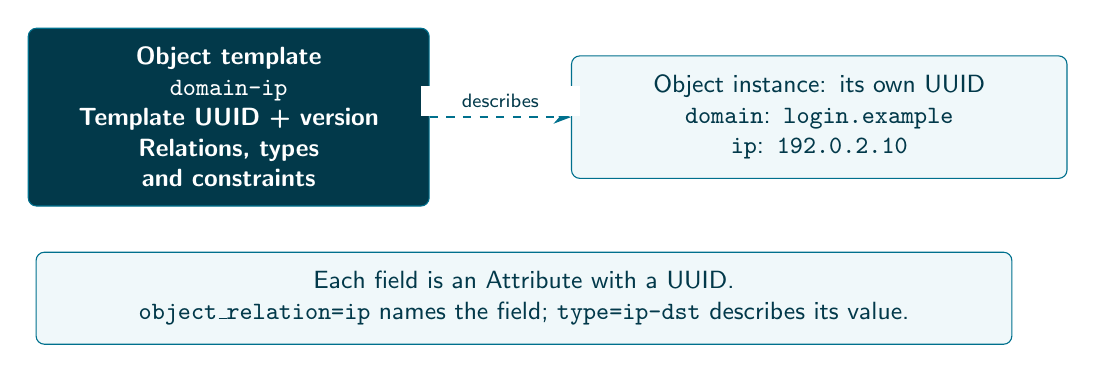
\begin{tikzpicture}
  \node[dm title,text width=4.6cm] (template) at (0,0)
    {Object template\\\texttt{domain-ip}\\Template UUID + version\\Relations, types and constraints};
  \node[dm box,text width=5.8cm] (instance) at (7.5,0)
    {Object instance: its own UUID\\\texttt{domain}: \texttt{login.example}\\\texttt{ip}: \texttt{192.0.2.10}};
  \draw[dm arrow,dashed] (template) -- node[dm label,above,text width=1.8cm] {describes} (instance);
  \node[dm box,text width=11.9cm] at (3.75,-2.3)
    {Each field is an Attribute with a UUID.\\\texttt{object\_relation=ip} names the field; \texttt{type=ip-dst} describes its value.};
\end{tikzpicture}
\par\endgroup
  \medskip
  Model one meaningful observation. Reuse a maintained template before inventing one.
  \note{The template UUID/version and object instance UUID have different purposes.
  Template definitions specify relation names, underlying attribute types, required
  alternatives and repetition. Relation ip commonly uses type ip-dst in domain-ip.
  A server can retain an object whose template is unavailable, but normal editing
  and conformity checks need a suitable definition. Enforcement differs by import
  path and client: inspect the actual template and validate the resulting instance.}
\end{frame}

\begin{frame}{Object references state a directed relationship}
  \begingroup\centering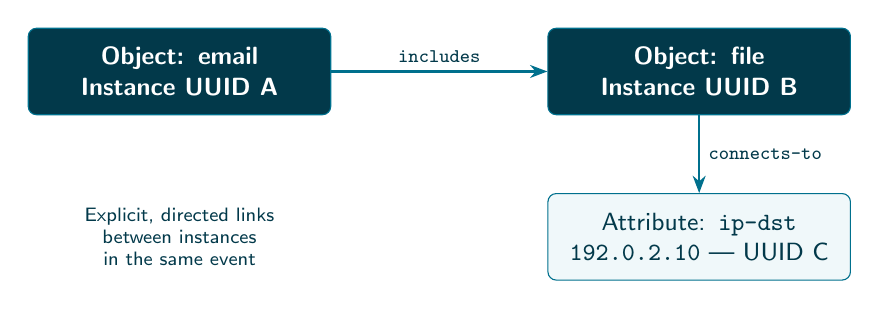
\begin{tikzpicture}
  \node[dm title] (email) at (0,0) {Object: email\\Instance UUID A};
  \node[dm title] (file) at (6.6,0) {Object: file\\Instance UUID B};
  \node[dm box] (ip) at (6.6,-2.1) {Attribute: \texttt{ip-dst}\\\texttt{192.0.2.10} --- UUID C};
  \draw[dm arrow] (email) -- node[dm label,above] {\texttt{includes}} (file);
  \draw[dm arrow] (file) -- node[dm label,right] {\texttt{connects-to}} (ip);
  \node[dm label,text width=3.4cm] at (0,-2.1)
    {Explicit, directed links\\between instances\\in the same event};
\end{tikzpicture}
\par\endgroup
  \begin{itemize}
    \item Source: an object instance. Target: an object or attribute.
    \item Store the relationship type and referenced instance UUID.
  \end{itemize}
  \note{This diagram models an email containing a file which connects to an IP.
  includes and connects-to are relationship labels, not object field names. Reverse
  direction changes the assertion. In the reviewed capture path, references resolve
  within the same event. The UI/API target-resolution path additionally allows
  authorised extension-to-parent references; availability depends on the path.
  Do not present ObjectReference as an arbitrary edge from
  any entity to any other entity. Analyst-data Relationships offer another mechanism
  for supported element types. Correlation requires no such explicit assertion.}
\end{frame}

\begin{frame}{Event Reports connect narrative to structured data}
  \begin{itemize}
    \item Keep the investigation story in Markdown inside the event.
    \item Reference attributes, objects and tags using MISP report syntax.
    \item Review the report's distribution and any sensitive prose.
  \end{itemize}
  \begin{block}{Illustrative report fragment}
    The message led to \texttt{@[attribute](<attribute-uuid>)}.\\
    The observation is recorded in \texttt{@[object](<object-uuid>)}.
  \end{block}
  \note{Angle-bracket UUIDs here are placeholders; insert real UUIDs from the event.
  These are MISP Markdown extensions, not ordinary Markdown links. A report has its
  own UUID and distribution and can inherit the event's distribution. Referencing
  an element is not a new ObjectReference or correlation. Redacting structured data
  alone may leave values in free text; inspect the actual report and export.}
\end{frame}

\begin{frame}{Identity survives sharing through UUIDs}
  \begin{tabular}{@{}L{.29\textwidth}L{.65\textwidth}@{}}
    \toprule
    Identifier & Purpose \\
    \midrule
    Local numeric ID & Locates a record on one MISP instance \\
    Element UUID & Identifies an event, attribute, object or other element across instances \\
    Template UUID + version & Identifies the definition used to describe an object \\
    Attribute value & Can match values in other records; does not identify the record \\
    \bottomrule
  \end{tabular}
  \medskip
  Preserve UUIDs when updating shared records; use new UUIDs for new observations.
  \note{Do not use a local database ID as a cross-instance identity. Two attributes
  may have different UUIDs but the same domain and may therefore correlate. A
  template UUID is not the UUID of any object instantiated from it. Reusing an
  element UUID for unrelated data risks replacing or confusing shared records.}
\end{frame}

\begin{frame}{Three ways to add context}
  \begingroup\centering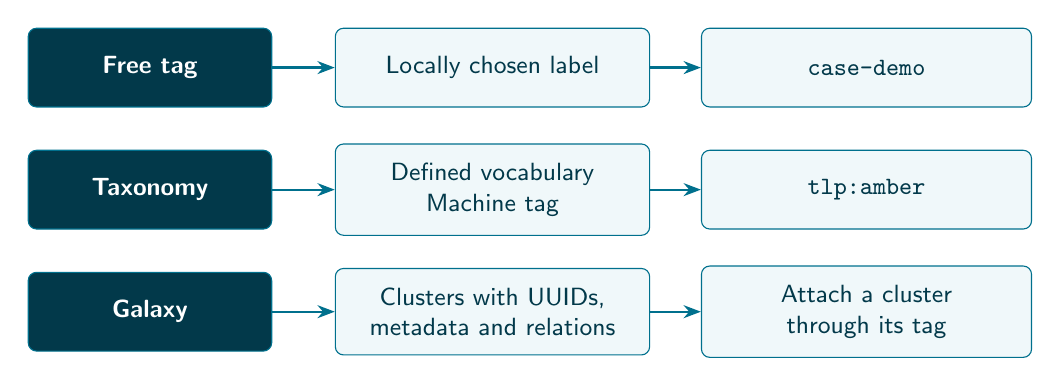
\begin{tikzpicture}
  \node[dm title,text width=2.6cm] (free) at (0,0) {Free tag};
  \node[dm box,text width=3.5cm] (freetag) at (4.35,0) {Locally chosen label};
  \node[dm box,text width=3.7cm] (freeexample) at (9.1,0) {\texttt{case-demo}};
  \draw[dm arrow] (free) -- (freetag); \draw[dm arrow] (freetag) -- (freeexample);
  \node[dm title,text width=2.6cm] (tax) at (0,-1.55) {Taxonomy};
  \node[dm box,text width=3.5cm] (taxtag) at (4.35,-1.55) {Defined vocabulary\\Machine tag};
  \node[dm box,text width=3.7cm] (taxexample) at (9.1,-1.55) {\texttt{tlp:amber}};
  \draw[dm arrow] (tax) -- (taxtag); \draw[dm arrow] (taxtag) -- (taxexample);
  \node[dm title,text width=2.6cm] (galaxy) at (0,-3.1) {Galaxy};
  \node[dm box,text width=3.5cm] (cluster) at (4.35,-3.1) {Clusters with UUIDs,\\metadata and relations};
  \node[dm box,text width=3.7cm] (attached) at (9.1,-3.1) {Attach a cluster\\through its tag};
  \draw[dm arrow] (galaxy) -- (cluster); \draw[dm arrow] (cluster) -- (attached);
\end{tikzpicture}
\par\endgroup
  \medskip
  A taxonomy defines labels. A galaxy organises richer concepts represented by clusters.
  \note{Free tags provide flexibility but require local conventions. Machine tags
  can follow namespace:predicate="value" or a simple namespace:predicate form,
  such as tlp:amber. A cluster is a record with identity and metadata, not simply a
  spelling variant of a free tag. Tag attachments connect clusters to event data.
  The diagram describes common usage and is not the complete taxonomy/galaxy schema.}
\end{frame}

\begin{frame}{Tag scope and handling must be explicit}
  \begin{itemize}
    \item Event tags describe the event; attribute tags describe specific data.
    \item Use the narrowest appropriate scope for confidence and classification.
    \item Local tag attachments stay local; shareable attachments can travel with data.
    \item A TLP label communicates handling expectations. Configure access separately.
  \end{itemize}
  \begin{block}{Avoid an inheritance assumption}
    Event context can be displayed or used by consumers without being copied into each attribute's tag list.
  \end{block}
  \note{The original overview said event context is propagated to underlying data.
  That is too broad for an interchange model. Inspect attachment scope, local flags
  and the selected export. Current MISP also supports Event Report tags; this slide
  highlights the common event/attribute distinction rather than enumerating all
  attachment types. A TLP tag alone is not a distribution setting or an ACL.}
\end{frame}

\begin{frame}{Galaxy clusters enrich classification}
  \begin{itemize}
    \item A galaxy groups a domain of knowledge: techniques, actors, tools, \ldots
    \item A cluster represents one concept with a UUID, description and metadata.
    \item Cluster relations can connect concepts, including across galaxies.
    \item Attach relevant clusters to the event or specific attributes.
  \end{itemize}
  \begin{block}{Example}
    Link the observed behaviour to a MITRE ATT\&CK technique cluster.\\
    Explain the evidence separately; a technique label alone does not establish attribution.
  \end{block}
  \note{Galaxy cluster metadata can contain external IDs, aliases and references.
  Standard collections and custom clusters have different maintenance and sharing
  workflows. Do not confuse galaxy cluster relations, ObjectReference or analyst
  Relationships. Use the Galaxy course for cluster updates and local/shareable
  attachments; avoid assuming a cluster is available on every recipient instance.}
\end{frame}

\begin{frame}{Analyst data preserves reasoning and assessments}
  \begingroup\centering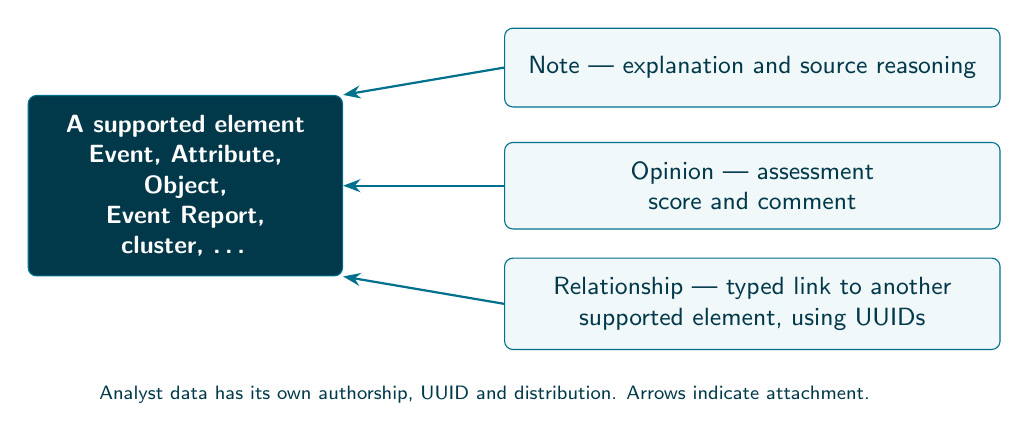
\begin{tikzpicture}
  \node[dm title,text width=3.5cm] (target) at (0,0)
    {A supported element\\Event, Attribute, Object,\\Event Report, cluster, \ldots};
  \node[dm box,text width=5.8cm] (note) at (7.2,1.5)
    {Note --- explanation and source reasoning};
  \node[dm box,text width=5.8cm] (opinion) at (7.2,0)
    {Opinion --- assessment score and comment};
  \node[dm box,text width=5.8cm] (relationship) at (7.2,-1.5)
    {Relationship --- typed link to another\\supported element, using UUIDs};
  \draw[dm arrow] (note.west) -- (target.north east);
  \draw[dm arrow] (opinion.west) -- (target.east);
  \draw[dm arrow] (relationship.west) -- (target.south east);
  \node[dm label] at (3.8,-2.65) {Analyst data has its own authorship, UUID and distribution. Arrows indicate attachment.};
\end{tikzpicture}
\par\endgroup
  \note{MISP 2.5 supports Note, Opinion and Relationship as analyst data. The
  reviewed valid targets also include Galaxy, Organisation, SharingGroup and analyst
  data itself; the picture intentionally shows common examples, not a full list.
  Opinion uses a 0--100 score; document what the score means in the workflow.
  Relationships carry source/target types and UUIDs plus a relationship label.
  Analyst data has separate distribution (0--4, no inherit-event value 5 in the
  reviewed model). Availability still depends on permissions and synchronisation
  support. Do not assume every note is shared with every reader of its target.}
\end{frame}

\begin{frame}{Sightings and proposals close the feedback loop}
  \begin{columns}[T,onlytextwidth]
    \column{.48\textwidth}
    \begin{block}{Sighting: feedback on an attribute}
      \texttt{0} --- sighting / observation\\
      \texttt{1} --- false-positive report\\
      \texttt{2} --- expiration
    \end{block}
    Include time and source. Visibility depends on the configured sighting policy.
    \column{.48\textwidth}
    \begin{block}{Proposal: suggested change}
      Suggest an attribute addition, modification or deletion for the event owner to review.
    \end{block}
    Record detailed reasoning in analyst data when appropriate.
  \end{columns}
  \note{Sightings attach to attributes, including object attributes. A positive
  sighting means observed, not necessarily malicious; false-positive and expiration
  records support later decisions. Bulk operations on an event do not turn sightings
  into generic event annotations. Proposals use ShadowAttribute and require an
  acceptance workflow; submitting a proposal does not immediately change the
  original. Keep sightings, proposals and analyst data conceptually separate.}
\end{frame}

\begin{frame}{Correlation reveals matches to investigate}
  \begingroup\centering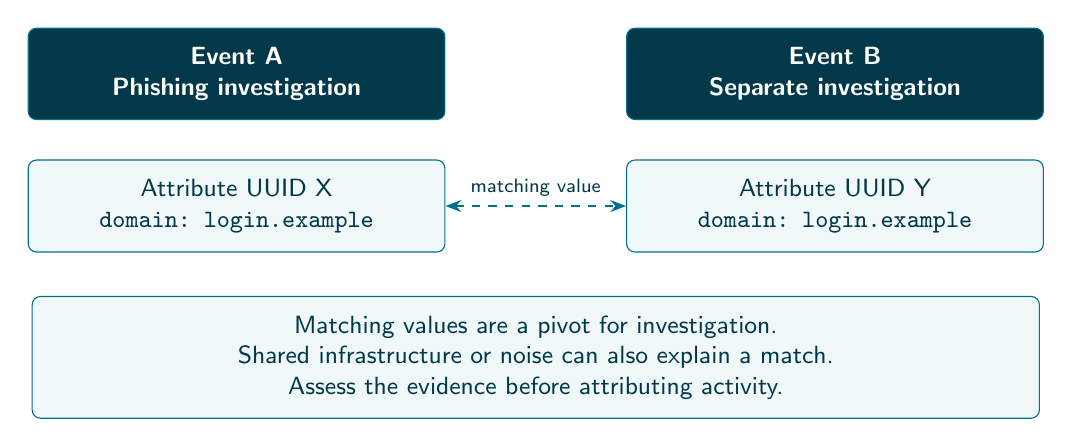
\begin{tikzpicture}
  \node[dm title,text width=4.8cm] (a) at (0,0) {Event A\\Phishing investigation};
  \node[dm title,text width=4.8cm] (b) at (7.6,0) {Event B\\Separate investigation};
  \node[dm box,text width=4.8cm,below=5mm of a] (aa)
    {Attribute UUID X\\\texttt{domain: login.example}};
  \node[dm box,text width=4.8cm,below=5mm of b] (bb)
    {Attribute UUID Y\\\texttt{domain: login.example}};
  \draw[dm match] (aa) -- node[dm label,above] {matching value} (bb);
  \node[dm box,text width=12.3cm] at (3.8,-3.6)
    {Matching values are a pivot for investigation.\\Shared infrastructure or noise can also explain a match.\\Assess the evidence before attributing activity.};
\end{tikzpicture}
\par\endgroup
  \note{The dashed bidirectional arrow denotes a computed match, not a stored
  directed assertion such as connects-to. Values are normalised and compared
  according to supported type/engine behaviour. Matching attributes may be
  standalone or inside objects. Permissions filter what a reader can see.
  Example values are synthetic and do not indicate malicious infrastructure.}
\end{frame}

\begin{frame}{Correlation depends on types and configuration}
  \begin{tabular}{@{}L{.17\textwidth}L{.38\textwidth}L{.38\textwidth}@{}}
    \toprule
    Mode & Example & Conditions \\
    \midrule
    Value match & Same eligible domain or hash & Type/engine rules and correlation enabled \\
    CIDR & \texttt{192.0.2.0/24} contains \texttt{192.0.2.10} & Advanced correlations enabled; supported IP types \\
    ssdeep & Similar fuzzy hashes & Advanced correlations, ssdeep runtime support and configured threshold \\
    \bottomrule
  \end{tabular}
  \medskip
  Non-correlating types, exclusions and over-correlation limits can suppress matches.
  \note{\raggedright The original slide misspelled CIDR as CDIR and suggested all attributes
  always correlate. In reviewed Correlation.php, advanced matching is gated by
  MISP.enable\_advanced\_correlations; ssdeep requires ssdeep\_fuzzy\_compare and uses
  MISP.ssdeep\_correlation\_threshold (fallback 40 in that source). Do not promise
  a threshold or fuzzy match without checking the instance. Attribute/event
  disable\_correlation, excluded values, engine selection and over-correlation
  handling also matter. to\_ids=false does not itself disable correlation.}
\end{frame}

\begin{frame}{Choose the right kind of link}
  \begin{tabular}{@{}L{.24\textwidth}L{.34\textwidth}L{.35\textwidth}@{}}
    \toprule
    Mechanism & Connects & Meaning \\
    \midrule
    Object relation & Object to its attribute field & \texttt{ip} names a field \\
    Object reference & Object to object / attribute & Explicit directed assertion \\
    Analyst Relationship & Supported elements by UUID & Analyst's typed assertion \\
    Cluster relation & Galaxy clusters & Knowledge-base relationship \\
    Correlation & Eligible matching attributes & Computed investigative pivot \\
    \bottomrule
  \end{tabular}
  \note{Ask which mechanism expresses an observed file contacting an address:
  an object reference is appropriate if modelled with a source file object and
  target attribute/object in the same event. Matching domains in separate events
  are correlation. Attaching an analyst's assessment of two supported entities is
  a Relationship. A field named ip is an object\_relation, not one of those edges.}
\end{frame}

\begin{frame}{Sharing settings constrain what leaves the event}
  \begin{itemize}
    \item Event distribution sets the containing audience; a sharing group can name it.
    \item Child settings can inherit where supported, or further restrict sharing.
    \item Check object, attribute, report and analyst-data settings separately.
    \item Check the actual recipient view and export, including free-text reports.
  \end{itemize}
  \begin{block}{Keep handling and access aligned}
    Distribution, sharing groups, permissions and sync/export settings enforce different parts of the workflow. Tags communicate context and handling.
  \end{block}
  \note{Avoid presenting child settings as a way to widen access beyond the parent.
  Event distribution uses 0 organisation, 1 community, 2 connected communities,
  3 all communities, 4 sharing group. Attributes/objects/reports also support
  5 inherit where applicable. Analyst data is a separate model; inspect its
  distribution and ACL rather than treating every element as an identical child.
  All communities is a distribution level, not anonymous public access. Validate
  with the intended non-admin recipient and outbound path. Publishing is not
  evidence that a recipient received the data or that old copies were recalled.}
\end{frame}

\begin{frame}{Keep event boundaries meaningful}
  \begin{itemize}
    \item Group observations that share an investigation, source or time context.
    \item Split unrelated incidents rather than building an unbounded indicator list.
    \item Use an extended event to add your perspective to a parent event.
    \item The extension retains its own identity, ownership and sharing settings.
  \end{itemize}
  \begin{block}{Extended event}
    The child event's \texttt{extends\_uuid} identifies the parent event.\\
    A combined view depends on the reader being allowed to see the relevant events.
  \end{block}
  \note{An extended event is not an edit to the parent's original records and does
  not bypass either event's visibility. Use it for complementary investigation
  context, not as a substitute for every correction proposal. Broad non-MISP feeds
  can introduce common shared values and noisy correlation: review grouping,
  provenance and selection before import. Size alone does not determine a useful
  event boundary.}
\end{frame}

\begin{frame}{Model a phishing observation}
  \begin{enumerate}
    \item Create an event for one investigation and define its audience.
    \item Add a \texttt{domain-ip} object for the domain and observed address.
    \item Add a standalone URL attribute if it has its own investigative role.
    \item Describe evidence in an Event Report; attach relevant context tags.
    \item Record an analyst Note and later sightings on the relevant attributes.
  \end{enumerate}
  \medskip
  Use \texttt{login.example} and \texttt{192.0.2.10} for discussion.\\
  Inspect correlations as leads; review \texttt{to\_ids} before consumer use.
  \note{Return to the event-anatomy diagram. This is a conceptual example, not an
  importable payload. An actual event requires valid UUIDs and appropriate fields;
  validate objects against the selected template. Keep documentation examples out
  of production detection. An object reference is optional: add one only when the
  investigation makes a meaningful directed assertion. Classification is not proof
  that the synthetic domain is malicious.}
\end{frame}

\begin{frame}{Exercise: choose an element and explain why}
  \begin{enumerate}
    \item A domain was observed resolving to two IP addresses in one observation.
    \item Another investigation contains the same domain.
    \item A file in this event contacted one of those addresses.
    \item A reviewer wants to explain doubts about the attribution.
    \item A recipient observed the domain yesterday.
    \item The event should be available only to a named community.
  \end{enumerate}
  \medskip
  Which choices express evidence, which express analysis, and which control access?
  \note{Expected discussion: (1) a suitable domain-ip object with repeated ip
  attributes, preserving observation context; (2) correlation if eligible/enabled,
  not proof of common actor; (3) file object reference connects-to an IP attribute
  or suitable target object in the same event; (4) Note, possibly Opinion with
  explanation, attached at the relevant scope; (5) type 0 Sighting on the domain
  attribute with time/source, not a maliciousness verdict; (6) event sharing-group
  distribution with reviewed membership, plus recipient/export verification.
  Ask why copying a TLP label alone does not solve item 6. Allow five minutes.}
\end{frame}

\begin{frame}{A useful record preserves meaning}
  \begin{itemize}
    \item Structure observations with attributes and coherent objects.
    \item Preserve narrative, provenance, UUIDs and observation times.
    \item Distinguish classification, asserted relationships and computed matches.
    \item Keep feedback and assessments attached to the right element.
    \item Verify the audience and payload before relying on sharing.
  \end{itemize}
  \note{A technically valid record can still be ambiguous or unsuitable for a
  consumer. Ask participants to explain one observation to another analyst using
  its model, evidence, time and sharing context. Continue with the full data-model,
  object-template, Galaxy, usage and API courses for deeper practice.}
\end{frame}

\begin{frame}{References and further training}
  \begin{itemize}
    \item \href{https://www.misp-standard.org/}{MISP standard}: exchange formats and schemas
    \item \href{https://www.circl.lu/doc/misp/}{MISP Book}: usage, sharing, analyst data and sightings
    \item \href{https://github.com/MISP/misp-objects}{MISP Objects}: maintained object definitions
    \item \href{https://github.com/MISP/misp-taxonomies}{MISP Taxonomies} and
      \href{https://github.com/MISP/misp-galaxy}{MISP Galaxy}: classification and context
    \item \href{https://github.com/MISP/MISP/tree/04fc5f8b7ccb52bb6614ca3e9ccdbfdf6585d985}{MISP 2.5.51 source reviewed}: model and correlation behaviour
  \end{itemize}
  \medskip
  Review date: 7 November 2026. Build instructions, review findings and source links are in the course README.
  \note{The README pins implementation references so future maintainers can audit
  claims. MISP's deployed version, engine and configuration affect behaviour.
  This update is a source/documentation review and PDF build validation, not a
  live-instance validation. Retain MISP/Team CIRCL attribution and the repository's
  AGPL-3.0-or-later or CC-BY-SA-4.0 licensing when adapting this deck.}
\end{frame}

\end{document}
